%/**
% * LaTeX thesis template (assumptions)
% * @author  : Alexander willner (willner@cs.uni-bonn.de)
% */

\cleardoublepage\chapter{Assumptions, Objectives and Scope}\minitoc\label{sec:assumptions}\vspace{.5cm}
\sidenote{text}
\noindent\lipsum[7]

\section{Use Cases and Assumptions}
\lipsum[5]

\section{Requirements and Objectives}
\lipsum[5]

\section{Test}

\cite{Waitzman:1999}

\small
\begin{equation}
  \begin{array}{l}
    \displaystyle t^{p_d}_{fw}(d) = max_{d}(t_{child_{i}}) \\
    \displaystyle t^{p_d}_{db}(d) = \sum_{i=1}^{d} t_{db_{i}} \\
    \displaystyle t^{p_d}_{pc}(n,d) =
    	\begin{cases}
        	t_{pc}(d) + c(n) & \text{if $d = 1$,}\\
        	t_{pc}(d) + c(n) + max(t_{avail}(d)) & \text{if $d>1$.}\\
        \end{cases}
  \end{array}
  \label{eq:var_idb}
\end{equation}
\normalsize

\begin{figure}
    \centering
    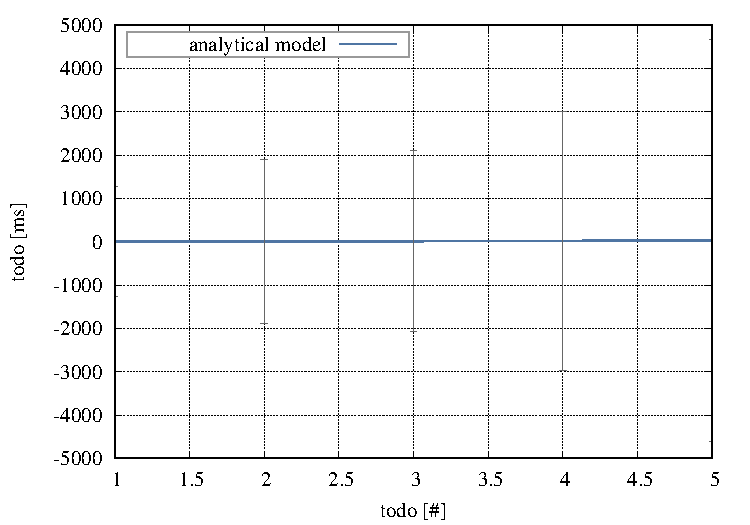
\includegraphics[width=.65\textwidth]{resources/images/example1.pdf}
    \caption{Example image.}
    \label{fig:example1}
\end{figure}

\begin{figure}
    \begin{subfigure}[b]{.5\textwidth}
      \centering
      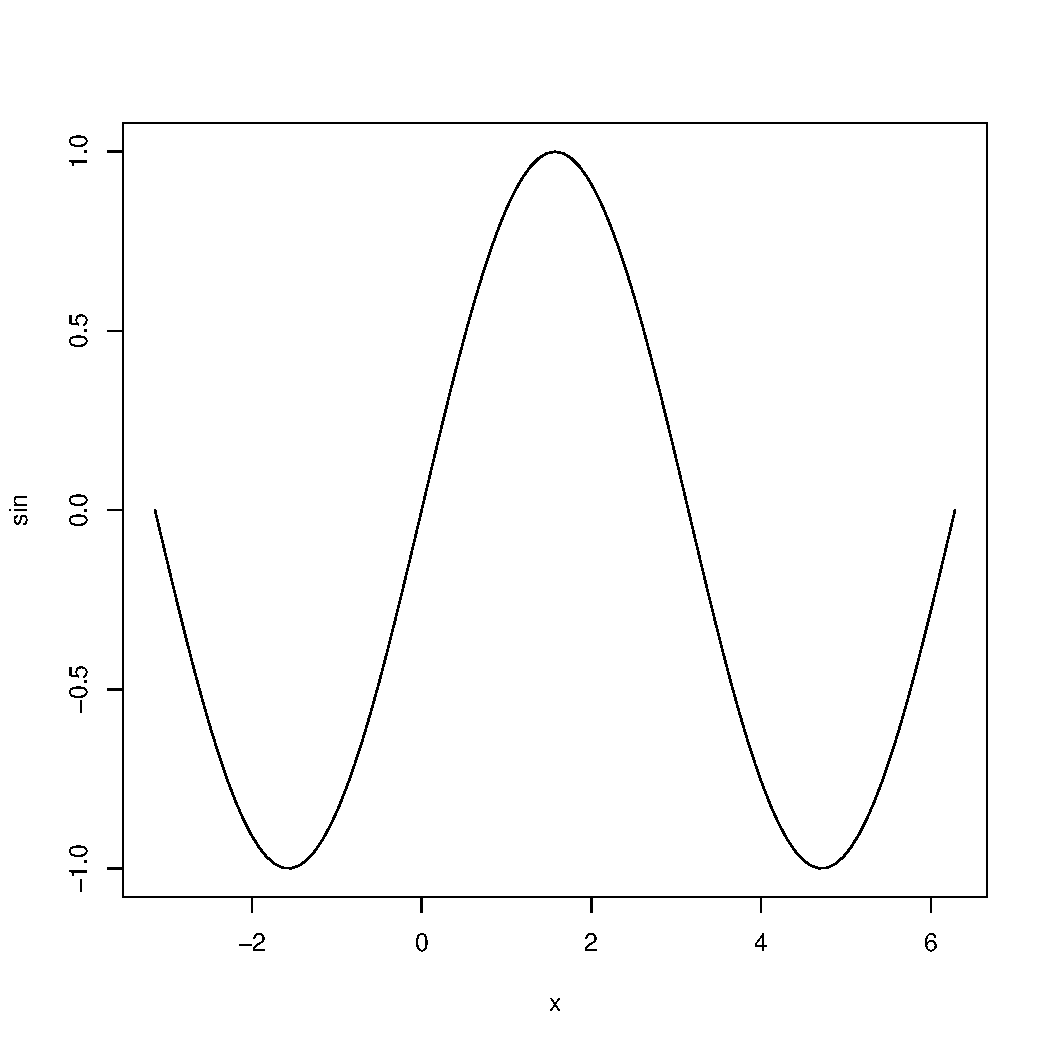
\includegraphics[width=.95\textwidth,frame]{resources/images/example2}
      \caption{example2}\label{fig:example2}
    \end{subfigure}~\begin{subfigure}[b]{.5\textwidth}
      \centering
      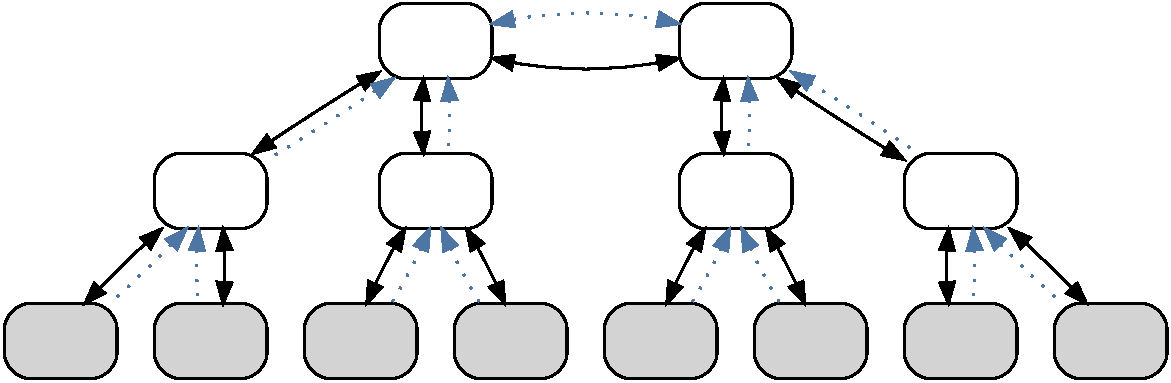
\includegraphics[width=.95\textwidth,frame]{resources/images/example3}
      \caption{example3}\label{fig:example3}
    \end{subfigure}
    \caption{Example images}\label{fig:exammple2_3}
\end{figure}

\begin{center}
  \begin{tabularx}{\textwidth}{ll}
      \caption{Example table}\label{tbl:exampletable}\\
        \toprule\textbf{Name} & \textbf{Age}\\\midrule
        \endfirsthead
        \toprule\textbf{Name} & \textbf{Age}\\\midrule
        \endhead
        \midrule
            \multicolumn{2}{r}{\emph{Continued on next page}}
        \endfoot
        \bottomrule
        \endlastfoot
       Hans           & 80             \\
       Heinrich       & 77             \\
       Herbert        & 84             \\
    \end{tabularx}
\end{center}

\lstset{language=Java, caption=Example Code., %
label=lst:example, numbers=left, stepnumber=1}
\lstinputlisting{resources/code/example.java}

\section{Summary}
\lipsum[5]
